\chapter{Použité metody}

% korelace
% ortogonální
% kontingencni tabulka (vicenasobna)

% zkrtky PCA, MCA, CA,
% znaceni jendotkový vektor rozměru J \mathbf{1}_J
% Singulární rozklad (zkratkou SVD podle anglického názvu Singular Value Decomposition) matice + singulární hodnoty
\section{Redukce dimenzionality} %Extrakce proměnných}

\subsection{Analýza hlavních komponent}


Analýza hlavních komponent (anglicky \emph{Principal component analysis}, dále jako PCA) je statistická metoda využívaná pro pro extrakci proměnných, redukci vícedimenzionálních dat nebo vizualizaci dat. Lze ji aplikovat pouze na kvantitativní data s numerickými, spojitými hodnotami, neboť metoda využívá lineární algebraické techniky, jako je například kovarianční matice, pro jejíž výpočet se předpokládají spojité hodnoty. 

Jednotlivá pozorování obsažená v datech bývají popsána několika různými proměnnými. Tyto proměnné jsou často vzájemně korelované a obsahují šum. Metoda PCA umožňuje extrahovat pouze důležité informace z proměnných a snížit šum.~k tomu je třeba vypočítat nové ortogonální proměnné, nazývané hlavní komponenty, které se získají jako lineární kombinace původních proměnných \cite{bib:PCA1}. Hlavní komponenty reprezentují směry největšího rozptylu původních dat a jsou řazeny podle své významnosti. Jinými slovy, první hlavní komponenta zachycuje co nejvíce variability v datech, druhá hlavní komponenta zachycuje co nejvíce variability, která nebyla zachycena první hlavní komponentou, pro zbylé komponenty analogicky. 
%, jinými slovy se jedná o přímku,  které nesou největší informaci o datech. Hlavní komponentu si lze představit jako novou osu, která umožňuje vidět data v takovém rozložení, že rozdíly mezi pozorováními jsou lépe patrné.  %https://builtin.com/data-science/step-step-explanation-principal-component-analysis

\subsubsection{Princip}

Předpokládáme množinu dat $X = (\bm{x}_1, \ldots, \bm{x}_N )$, kde $N$ j počet pozorování a každý vektor $\bm{x}_i$ přísluší jednomu pozorování popsanému $M$ proměnnými. $\mathbf{X}$ je potom matice rozměru $N\times M$ vstupních dat. Dále je definovaný výběrový průměr $\bar{\bm{x}}$ jako
\begin{equation}
    \bar{\bm{x}} = \frac{1}{N} \sum_{i=1}^{N} \bm{x}_i,
\end{equation}
a výběrová kovarianční matice $\mathbf{C}$

\begin{equation}
    \mathbf{\mathbf{C}} = \frac{1}{N} \sum_{i=1}^{N} (\bm{x}_i - \bar{\bm{x}}).
\end{equation}

První hlavní komponentu, která popisuje největší rozptyl dat označíme $y_{1i}$ a vypočteme následovně jako lineární kombinaci původních proměnných
\begin{equation}
    y_{1i} = \bm{a}_1^\top (\bm{x}_i - \bar{\bm{x}}), \quad \mbox{pro } i=1,\ldots,N,
\end{equation}
kde $\bm{a}_1 = (a_{11}, \ldots, a_{M1})^\top $ je vektor vah. 

Optimální vektor $\bm{a}_1$ je takový vektor, který maximalizuje výběrový rozptyl nové proměnné $y_{1i}$ za podmínky $\bm{a}_1^\top\bm{a}_1 = 1$. Pakliže je výběrový rozptyl $y_{1i}$ definován jako 
\begin{equation}
    D(y_{11}, \ldots, y_{1N}) = \bm{a}_1^\top \mathbf{C} \bm{a}_1
\end{equation}
můžeme maximalizační úlohu vyřešit pomocí metody Lagrangeových multiplikátorů. Lagrageova funkce s parametrem $\lambda_1$ má následující tvar
\begin{equation}
    \mathcal{L}(\bm{a}_1, \lambda_1) = \bm{a}_1^\top \mathbf{C} \bm{a}_1 - \lambda_1(\bm{a}_1^\top\bm{a}_1 - 1).
\end{equation}

Derivaci funkce položíme rovnou nule 
\begin{align*}
    \frac{\partial \mathcal{L}}{\partial \bm{a}_1}  = 2 \mathbf{C} \bm{a} - 2\lambda_1 \bm{a}_1 \overset{!}{=}  0 \\
    (\mathbf{C} - \lambda_1 \mathbf{I} ) \bm{a}_1 \overset{!}{=}  0,  \\
\end{align*}
kde $\mathbf{I}$ je jednotková matice.

Řešíme soustavu lineárních rovnic pro neznámý parametr $\bm{a}_1$, která má řešení právě tehdy, když je matice $\mathbf{C} - \lambda_1 \mathbf{I} $ singulární, tedy platí, že její determinant  je roven nule. $\lambda_1$ je pak největší vlastní číslo matice $\mathbf{C}$ a $\bm{a}_1$ vlastní vektor příslušný tomuto vlastnímu číslu. Toto tvrzení se matematicky zapíše následovně
\begin{equation}
    \mathbf{C} \bm{a}_1 = \lambda_1 \bm{a}_1. \\
\end{equation}
Po vynásobení vektorem $\bm{a}_1$ zleva získáme řešení pro maximální rozptyl proměnné $y_{1i}$
\begin{equation}
    D(y_{11}, \ldots, y_{1N}) = \bm{a}_1^\top \mathbf{C} \bm{a}_1 = \lambda_1.
\end{equation}


Druhá hlavní komponenta
\begin{equation}
    y_{2i} = \bm{a}_2^\top (\bm{x}_i - \bar{\bm{x}}), \quad \mbox{pro } i=1,\ldots,N,
\end{equation}
se vypočte obdobným způsobem s přidanou podmínkou ortogonality vzhledem~k první hlavní komponentě -- druhá hlavní komponenta nesmí být korelovaná s předchozí, první hlavní komponentou. Potom popisuje druhý největší možný rozptyl v datech. Znázornění dvou hlavních komponent ve dvoudimenzionálním prostoru je vyobrazeno na obrázku \ref*{obr:met:PCA1}.
Vektor  $\bm{a}_2$ se opět získá jako jednotkový vlastní vektor kovarianční matice $\mathbf{C}$ příslušící druhému největšímu vlastnímu číslu $\lambda_2$.\cite{bib:PCA1} %https://builtin.com/data-science/step-step-explanation-principal-component-analysis

\begin{figure}[hbtp!]
    \centering
    % 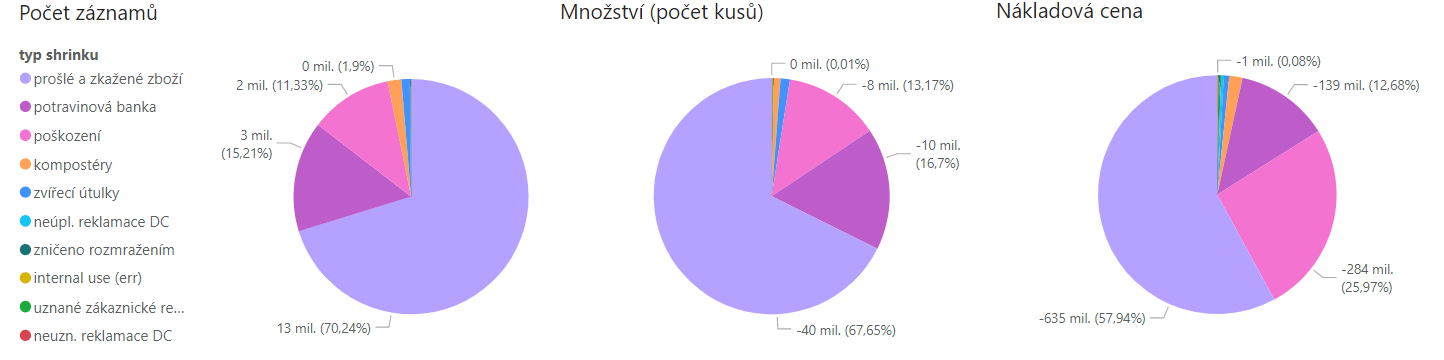
\includegraphics[width=\textwidth]{obrazky/grafy/Graf_celkem-D.png}
    \caption{Znázornění dvou hlavních komponent na dvoudimenzionálních datech.}
    \label{obr:met:PCA1}
\end{figure}


Získání předpisů pro další hlavní komponenty je analogické. Obecně lze zapsat metodu PCA a převod původních proměnných následujícím maticovým zápisem
\begin{equation}
    \mathbf{Y} = \mathbf{XA}, 
\end{equation}
kde $\mathbf{X}$ je matice vstupních dat, $\mathbf{A}$ je matice vlastních vektorů kovarianční matice $\mathbf{C}$. Pro matici $\mathbf{A}$ zároveň platí $\mathbf{C} =  \mathbf{A} \mathbf{\Lambda} \mathbf{A}^\top$, kde $\mathbf{\Lambda}$ je diagonální matice vlastních čísel $\mathbf{C}$.\cite{bib:PCA2}  %wikipedia

\subsection{Korespondenční analýza}

Vícenásobná korespondenční analýza (anglicky \emph{Multiple correspondence analysis}, dále jako MCA) je metoda, která umožňuje popsat vztahy mezi daty, které jsou popsané kategorickými proměnnými, vytvořením kontingenční tabulky. V případě, že se popisuje vzájemná relace pouze dvou proměnných, se použije základní korespondenční analýza\footnote{anglicky \emph{correspondence analysis} (CA)}. MCA je alternativou~k PCA, pokud jsou analyzovanými daty kategorická data. \cite{bib:MCA1}

% \subsubsection{Princip korespondenční analýzy}
\subsubsection{Značení}
%https://statmath.wu.ac.at/courses/CAandRelMeth/caipA.pdf
Nechť $\mathbf{N}$ typu $I\times J$ je matice dat, kde I odpovídá počtu pozorování a J je počet kategorií. %asi pocet kategorii, najit !!!
Matice $\mathbf{N}$ je převedena na korespondenční matici $\mathbf{P}$ vydělením matice $\mathbf{N}$ jejím celkovým součtem $n = \sum_{i=1}^{I} \sum_{j=1}^{J} n_{ij}=\mathbf{1}^\top_I \mathbf{N}\mathbf{1}_J$. To zaručuje, že součet prvků matice $\mathbf{P}$ je roven jedné. Tyto kroky lze shrnout následujícím matematickým zápisem
\begin{equation}
    \mathbf{P} = \frac{1}{n}\mathbf{N}, \qquad \mathbf{P} = \{p_{ij}\},  \qquad  \sum_{i=1}^{I} \sum_{j=1}^{J} p_{ij} = 1.
\end{equation}
Součet $i$tého řádku, resp. součet $j$tého sloupce je značen následovně
\begin{align*}
    r_i = \sum_{j=1}^{J} \qquad \mbox{ pro } i=1,\ldots,I, \\
    c_j = \sum_{i=1}^{I} \qquad \mbox{ pro } j=1,\ldots,J.
\end{align*}
Vektor $\bm{r} = \mathbf{P} \mathbf{1}_J $ obsahuje všechny řádkové součty matice $\mathbf{P}$, analogicky vektor $\bm{c} = \mathbf{P}^\top \mathbf{1}_I $ obsahuje všechny sloupcové součty téže matice.

Pro další výpočty zavedeme značení pro diagonální matice, které mají na diagonále  řádkový, resp. sloupcový součet
\begin{equation}
    \mathbf{D}_r = \mbox{diag}(\bm{r}), \quad \mbox{ resp. } \quad \mathbf{D}_c = \mbox{diag}(\bm{c}).
\end{equation}

% Pro připomenutí je vhodné dodat, že součet matice P je jedna

\subsubsection{Výpočetní algoritmus}\cite{bib:CA1}
Označme $\mathbf{S}$ následující matici
\begin{equation}
    \mathbf{S} := \mathbf{D}_r^{-\frac{1}{2}} (\mathbf{P} - \bm{rc}^\top) \mathbf{D}_c^{-\frac{1}{2}}.
\end{equation}
Po té proveďme singulární rozklad této matice
\begin{equation}
    \mathbf{S} = \mathbf{U}\mathbf{\Delta}\mathbf{V}^\top,
\end{equation}
kde $\mathbf{U}^\top\mathbf{U}=\mathbf{V}^\top\mathbf{V}=\mathbf{I}$ a $\mathbf{\Lambda} = \mathbf{\Delta}^2$ je matice vlastních čísel.
